\chapter{Implementation}
\label{implementation}
In diesem Kapitel wird die Implementation des Projekts beschrieben. Auf Basis der beschriebenen Konzeption wird im Anschluss die Implementation erfolgen. 
\section{Kommunikation}
Da die Kommunikation des verteilten Systems nachrichtenbasiert geschieht, ist der Entwurf eigener Nachrichtenstrukturen notwendig. Die Kommunikation zwischen dem Master den Workern findet mit Hilfe der Nachrichten statt. Konkret handelt es sich nach \citep{tanenbaum} bei der gewählten Architektur um eine \emph{Message-Queue-Architektur}. \\
Zur Strukturierung fiel die Wahl auf das Nachrichtenaustauschformat \enquote{JavaScript Object Notation} oder kurz \emph{JSON}, da dieses Format sehr leichtgewichtig und vollständig anpassbar ist. Zudem ist die Maschinenlesbarkeit im Vergleich zu XML einfacher umzusetzen, da zur Interpretation von XML eigene Schemata entwickelt werden müssten. \\
Als Kommunikationsplattform wird ein Node-Server benutzt, da dieser für den vorgesehenen Bereich schnell einsetzbar und mit dem JSON-Format kompatibel ist. Der Webserver basiert auf dem Javascript-Framework Node.js und ist für die Verteilung der Nachrichten zwischen den Rechnern des verteilten Systems verantwortlich. \\

Um Rückschlüsse auf die Geschwindigkeit verschiedener Hash-Algorithmen schließen zu können, kann bei Start der Applikation zwischen verschiedenen Hash-Algorithmen gewählt werden. Zur Auswahl stehen die Hash-Algorithmen \emph{MD5}, \emph{SHA 128} sowie \emph{SHA 256}. Die Geschwindigkeitsunterschiede beruhen primär auf der unterschiedlichen Schlüssellänge der jeweiligen Algorithmen.\\


Nachfolgend werden die entwickelten Nachrichtenstrukturen und deren Inhalt beschrieben. Zum besseren Verständnis werden die Nachrichten in die Senderichtungen zum Worker oder zum Master strukturiert. \\
Auf programmatischer Ebene wird zudem zwischen \emph{Basic Messages} und \emph{Extended Messages} unterschieden. Basic Messages beinhalten den Status des sendenden Rechners und maximal einen weiteren Wert, während Extended Messages neben dem Status mehrere Werte beinhalten. Durch diese Strukturierung ist ein effektives Messageparsing möglich. 

\subsection{Asynchronität}
Die Kommunikation innerhalb des verteilten Systems wird durch den Master sichergestellt. Konkret werden die Nachrichten durch den NODE-Server an alle Rechner des verteilten Systems (Broadcast) versendet. Dies bedeutet, dass jeder Rechner alle Nachrichten erhält und lokal zur Verfügung stehen. Damit die jeweiligen Rechner die Nachrichten zuordnen können, werden die Funktionen \emph{decideWhatToDoBasicMessage} und \emph{decideWhatToDoExtendedMessage} implementiert. Diese unterscheiden, wie der Name bereits vermuten lässt, zwischen \emph{Basic Messages} und \emph{Extended Messages}. Aber auch bei Master und Worker sind die Funktionen unterschiedlich implementiert, da diese unterschiedlich auf die Nachrichten reagieren. \\
Die Funktionen treffen ihre Entscheidungen auf Basis des Nachrichtenheaders sowie des Ziels der Nachricht, wie in den folgenden Codefragmenten zu erkennen ist. 
\newpage

\texttt{Klasse MasterOperation.swift}
\begin{lstlisting}[basicstyle=\ttfamily,numbers=left,numberstyle=\footnotesize\ttfamily,backgroundcolor=\color{sourcegray}]
func decideWhatToDoBasicMessage(message:BasicMessage){
	let messageHeader = message.status
        
    switch messageHeader {
        case MessagesHeader.newClientRegistration:
            newClientRegistration(message)
            break
        case MessagesHeader.alive:
            alive(message)
            break
        default:
            break
    }
}


func decideWhatToDoExtendedMessage(message:ExtendedMessage){
    let messageHeader = message.status
        
    switch messageHeader {
        case MessagesHeader.hitTargetHash:
            hitTargetHash(message)
            break
        case MessagesHeader.hashesPerTime:
            hashesPerTime(message)
            break
        case MessagesHeader.finishedWork:
            finishedWork(message)
            break
        default:
            break
    }
}
\end{lstlisting}

\newpage

\texttt{Klasse WorkerOperation.swift}
\begin{lstlisting}[basicstyle=\ttfamily,numbers=left,numberstyle=\footnotesize\ttfamily,backgroundcolor=\color{sourcegray}]
func decideWhatToDoBasicMessage(message:BasicMessage){
   let messageHeader = message.status
        switch messageHeader {
        case MessagesHeader.stillAlive:
            stillAlive(message)
            break
        case MessagesHeader.stopWork:
            stopWork()
            break
        default:
            break
    }
}

func decideWhatToDoExtendedMessage(message:ExtendedMessage){
    let messageHeader = message.status
    
    switch messageHeader {
        case MessagesHeader.setupConfig:
            setupConfig(message)
            break
        case MessagesHeader.newWorkBlog:
            newWorkBlog(message)
            break
        default:
            break
     }
}
\end{lstlisting}

Dieses Vorgehen hat den Vorteil, dass die Verarbeitung der Nachrichten asynchron geschehen kann. Durch die asynchrone Verarbeitung kann die Performance des verteilten Systems deutlich gesteigert werden, da die Rechner unabhängig voneinander arbeiten können. \\
Die Nachrichten werden in Warteschlangen (Queues) gespeichert. Durch den Einsatz von \emph{GrandCentralDispatch (GCD)}\footnote{\url{https://developer.apple.com/library/ios/documentation/Performance/Reference/GCD_libdispatch_Ref/index.html}} wird die Verteilung von Threads auf verschiedene Prozessorkerne vom Betriebssystem übernommen. Durch diese Abstraktion ist für den Entwickler eine effektivere Verteilung von Threads möglich. Da die Erstellung von Queues durch das Grand Central Dispatch realisiert wird, ist die Verteilung im verteilten System effizient möglich. Das GCD legt die Queues in Threads ab und übernimmt deren Verteilung. Zudem unterstützt GCD die Prozessverteilung auf Ebene des Betriebssystems.\\
Um die Performance weiter zu steigen, sollen die erstellten Threads eine hohe Priorität erhalten, um vom Betriebssystem bevorzugt bearbeitet zu werden. Die Zuweisung einer hohen Priorität unter GCD ist allerdings nur über einen Umweg möglich, da hohe Prioritäten nur für bestimmte Systemdienste vorgesehen sind. Mit folgendem Programmcode können die Nachrichten-Warteschlangen dennoch mit einer hohen Priorität versehen werden:


\texttt{Klasse WorkerOperation.swift}
\begin{lstlisting}[basicstyle=\ttfamily,numbers=left,numberstyle=\footnotesize\ttfamily,backgroundcolor=\color{sourcegray}]
  let queue = dispatch_queue_create
  ("\(Constants.queueID).compareHashes", nil)
  
  let highPriority = 
  dispatch_get_global_queue(DISPATCH_QUEUE_PRIORITY_HIGH, 0)
  
  dispatch_set_target_queue(queue, highPriority)
  
  
  
  dispatch_async(queue) {
     _ = passwordArray.map { password in
     
     let passwordQueue = 
     dispatch_queue_create("\(Constants.queueID).
     \(password)", nil)
\end{lstlisting}

Des weiteren wird die Parallelisierung weiter ausgebaut, indem die Queues, in denen sich die Passwortblöcke befinden, auf den einzelnen Workern weiter  aufgeteilt werden. Ein Beispiel dazu lässt sich ebenfalls aus dem Programmcode entnehmen. \\

\begin{figure}[!ht]
	\centering
		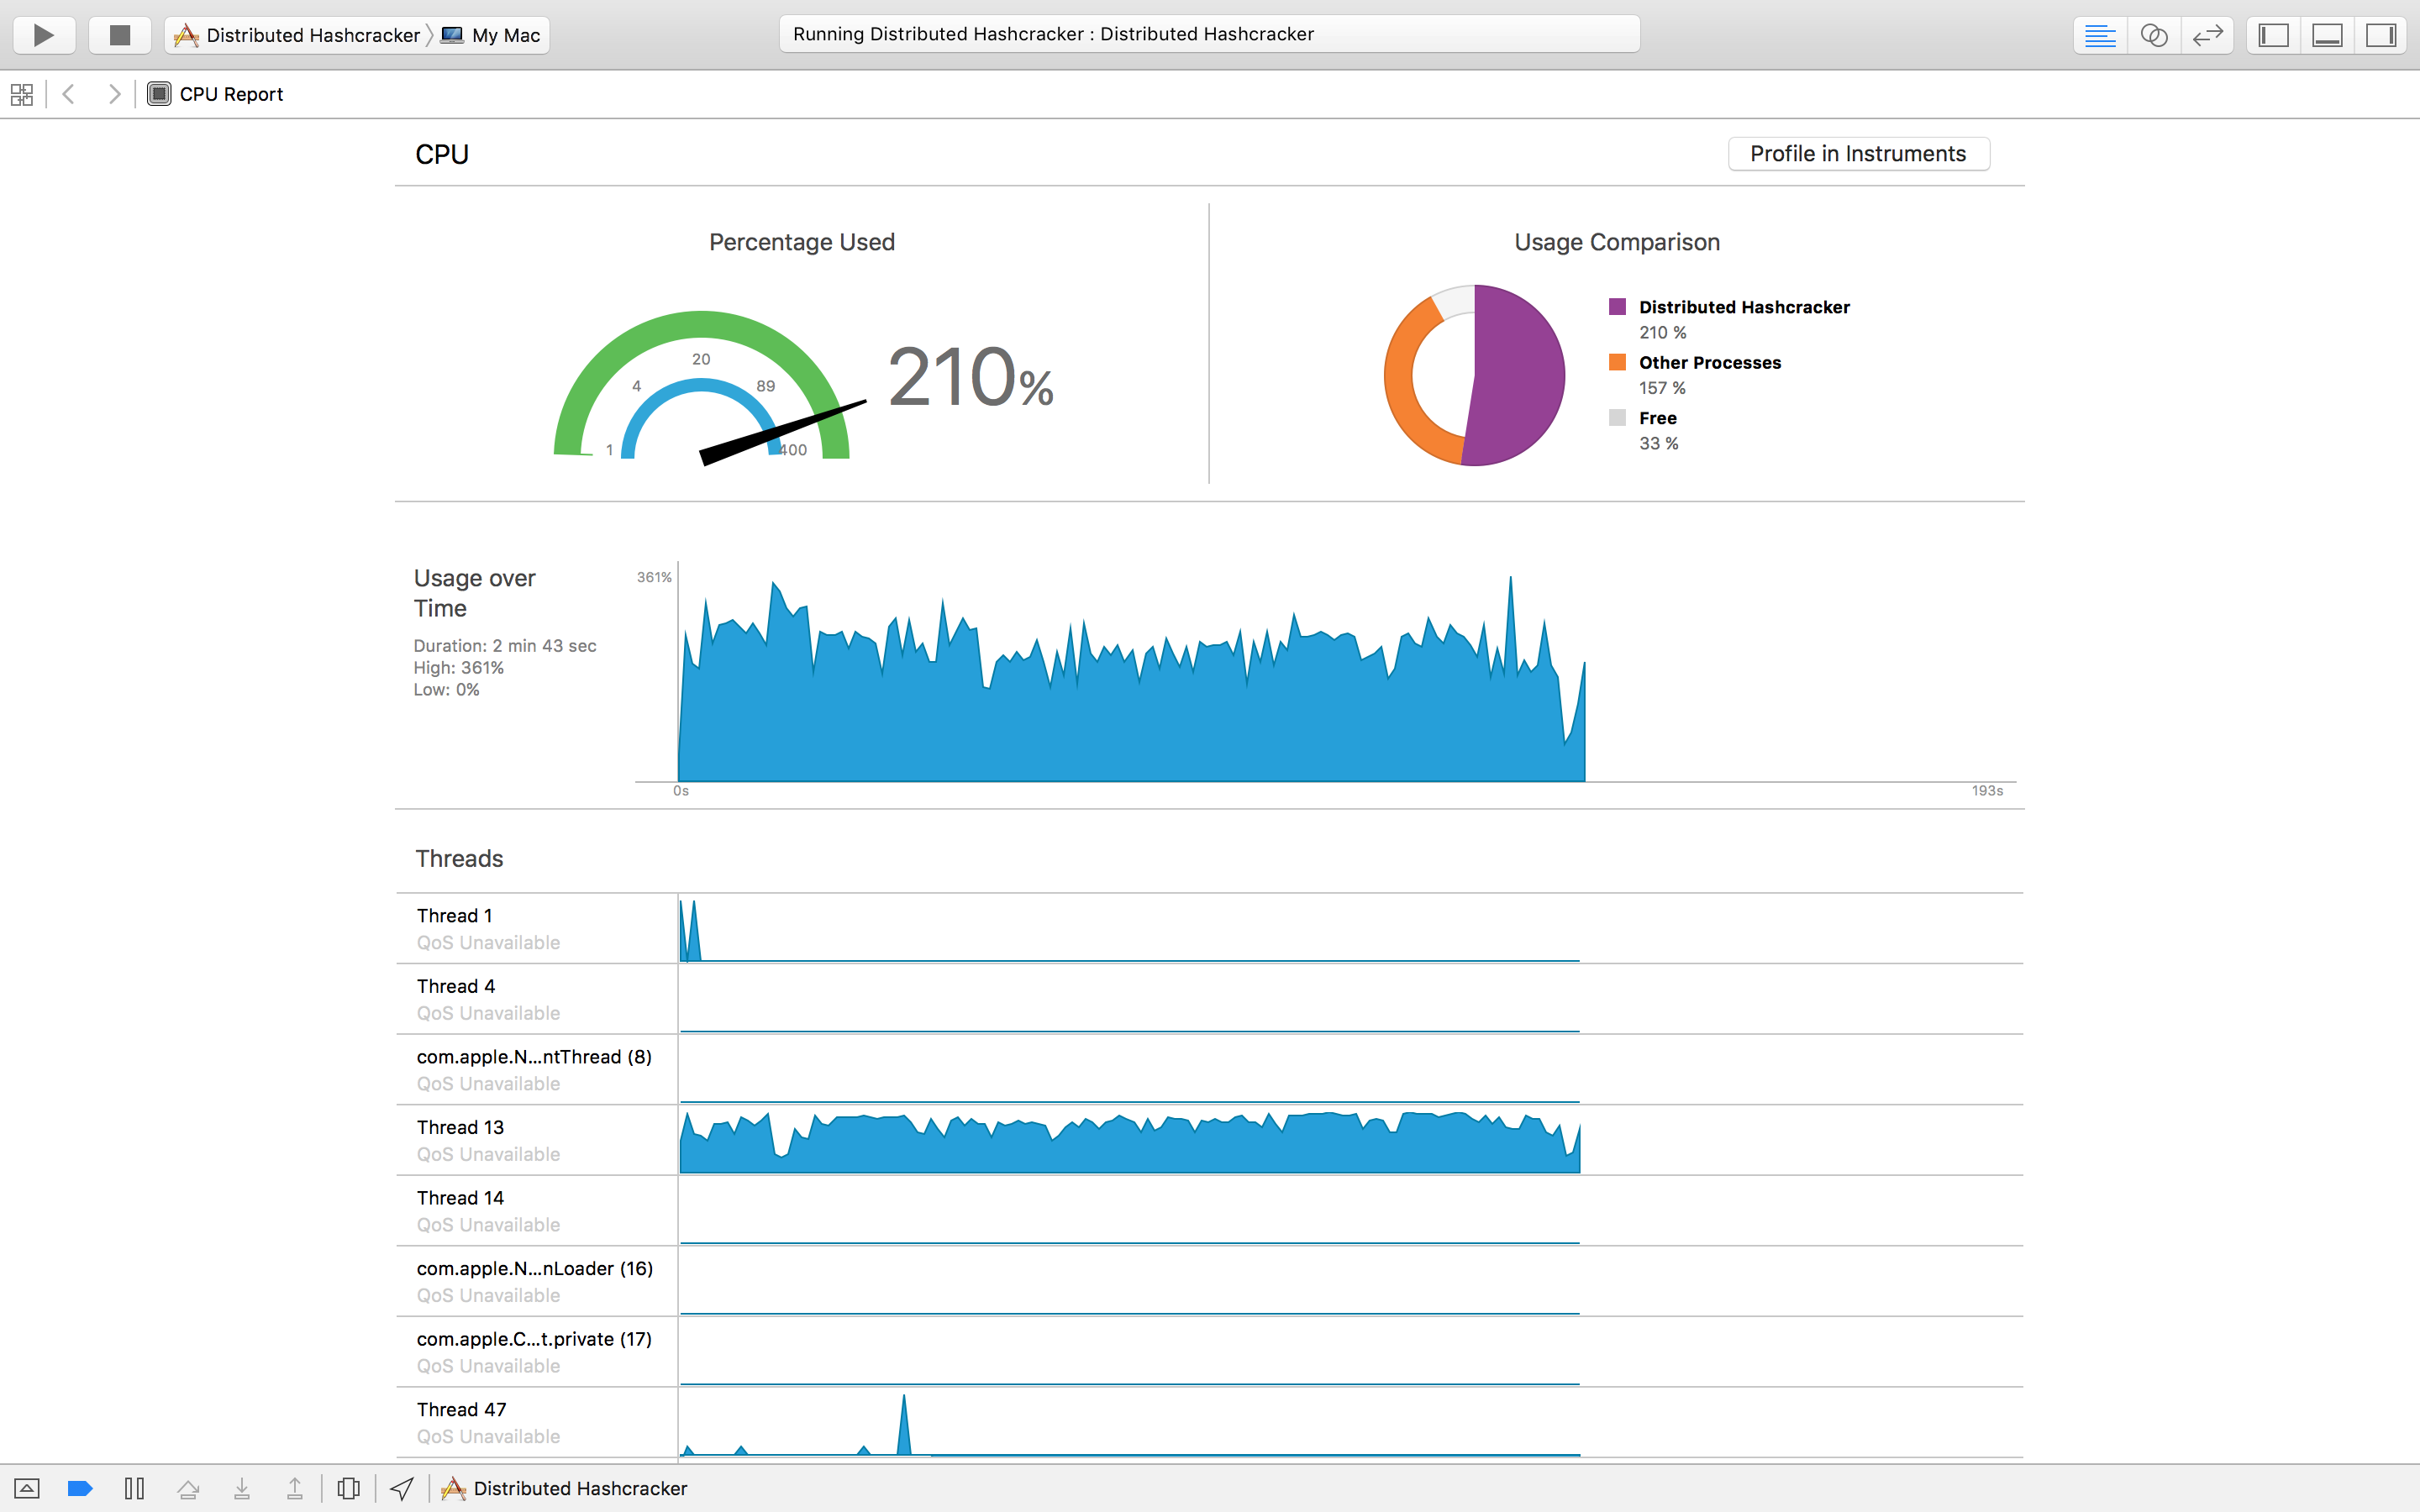
\includegraphics[natwidth=1200pt, natheight=349pt, width=1.0\textwidth]{images/screenshot_cpu.png}
	\caption{Verlauf der CPU-Auslastung während der Laufzeit, gemessen in Xcode mit zwei Prozessorkernen.}
	\label{fig:screenshotCPU}
\end{figure}


Grafik \ref{fig:screenshotCPU} zeigt, dass die zwei verfügbaren Prozessorkerne (ein Kern entspricht einer Auslastung von 100\%) mit der implementierten Verteilungsstrategie effektiv genutzt werden. Zur Messung wurde die Entwicklungsumgebung \emph{Xcode} genutzt. 

\subsection{Lenses}
Threadsicherheit bedeutet, dass Softwarekomponenten problemlos von verschiedenen Bereichen genutzt werden können, ohne dass dabei Nebeneffekte auftreten. Damit ist Threadsicherheit implizit wichtiger Bestandteil eines verteilten Systems. \\
Die Arbeitspakete (\emph{Work Blogs}) werden in \emph{WorkBlogQueues} gespeichert. Diese Queues beinhalten Arrays. Da Arrays in der Programmiersprache \emph{Swift} standardmäßig nicht threadsicher sind, werden sogenannte \emph{Lenses} eingesetzt. \\
Lenses stellen Getter- und Setter-Methoden zur Verfügung. 

\texttt{Klasse Lens}
\begin{lstlisting}[basicstyle=\ttfamily,numbers=left,numberstyle=\footnotesize\ttfamily,backgroundcolor=\color{sourcegray}]
struct Lens<Whole, Part> 
{
	let get : Whole -> Part
	let set: (Part, Whole) -> Whole
}
\end{lstlisting}

Die Getter-Methode ruft dabei einen Teil (Part) \enquote{des Ganzen (Whole)} ab, während die Setter-Methode aus einem Part und einem Whole ein \enquote{neues Ganzes (Whole)} erzeugt. \\
Mit Hilfe dieser Methode kann mit konstanten Arrays gearbeitet werden, um die Threadsicherheit herzustellen. Dabei werden die Daten in konstanten Arrays abgelegt. Muss ein Eintrag bearbeitet werden, wird mit Hilfe der Getter-Methode ein konstantes Array aufgerufen. Die Inhalte können nun über die Setter-Methode bearbeitet und in ein neues, konstantes Array geschrieben.\\
Folgender Programmcode zeigt eine konkrete Implementierung von Lenses:

\texttt{Klasse MessageQueue}
\begin{lstlisting}[basicstyle=\ttfamily,numbers=left,numberstyle=\footnotesize\ttfamily,backgroundcolor=\color{sourcegray}]
func get() -> Message? {
	dispatch_semaphore_wait
	(semaphore, DISPATCH_TIME_FOREVER)
	guard let firstElement = messagesLens.
	get(messages).first else {
		dispatch_semaphore_signal(semaphore)
        return nil
	}
        
	messages = messagesLens.set([], 
	messages.dropFirst().map{ $0 })
	dispatch_semaphore_signal(semaphore)
            
	return firstElement
    }
\end{lstlisting}

\subsection{Nachrichten zum Worker}
In diesem Abschnitt werden die Strukturen beschrieben, welche vom steuernden Rechner (Master) zu einem der Worker gesendet werden.\\

\texttt{SetupAndConfig(Extended Message)}
\begin{lstlisting}[basicstyle=\ttfamily,numbers=left,numberstyle=\footnotesize\ttfamily,backgroundcolor=\color{sourcegray}]
{
  "status" : "setupConfig",
  "value" : {
    "algorithm" : "#HASH_ID",
    "target" : "#TARGET_HASH", 
    "worker_id" : "#WORKER_ID"
  }
}
\end{lstlisting}
Ein im Cluster neu hinzugefügter Worker erhält seine Konfigurationsparameter, damit dieser als Worker im verteilten System genutzt werden kann. 
Der Wert \textbf{algorithm} übergibt die ID des Hash-Algorithmus, welcher in der aktuellen Passwortberechnung benutzt wird. \textbf{Target} übermittelt den Hash des Zielpasswortes. Die \textbf{workerID} ist der vom Master vorgegebene Hostname oder die IP-Adresse, die den Workern mitgeteilt werden muss.\\

\texttt{getWork (Extended Message)}
\begin{lstlisting}[basicstyle=\ttfamily,numbers=left,numberstyle=\footnotesize\ttfamily,backgroundcolor=\color{sourcegray}]
{
  "status" : "newWorkBlog",
  "value" : {
    "worker_id" : "#WORKER_ID"
    "hashes" : ["#NEW_HASHES"]
  }
}
\end{lstlisting}
Der Worker erhält durch einen neuen WorkBlog, den dieser abarbeiten wird.\\

\texttt{Stop Work (Basic Message)}
\begin{lstlisting}[basicstyle=\ttfamily,numbers=left,numberstyle=\footnotesize\ttfamily,backgroundcolor=\color{sourcegray}]
{
  "status" : "stopWorking",
  "value" : ""]
  }
}
\end{lstlisting}
Durch \enquote{stopWork} wird den Workern mitgeteilt, dass diese die Berechnungen stoppen können. Dies ist in der Regel der Fall, wenn das Zielpasswort identifiziert wurde. \\


\texttt{stillAlive (Basic Message)}
\begin{lstlisting}[basicstyle=\ttfamily,numbers=left,numberstyle=\footnotesize\ttfamily,backgroundcolor=\color{sourcegray}]
{
  "status" : "stillAlive",
  "value" : ""
}
\end{lstlisting}
Mit Hilfe dieser Nachricht fragt der Master an, ob die angesprochenen Worker noch verfügbar sind. Wenn diese nicht antworten, werden sie der Liste der verfügbaren Worker (Worker Queue) entfernt. 

\pagebreak

\subsection{Nachrichten zum Master}
Folgende Nachrichten werden von den Workern an die Master gesendet. \\

\texttt{newClientRegistration (Basic Message)}
\begin{lstlisting}[basicstyle=\ttfamily,numbers=left,numberstyle=\footnotesize\ttfamily,backgroundcolor=\color{sourcegray}]
{
  "status" : "newClientRegistration",
  "worker" : "#WORKER_ID"
}
\end{lstlisting}
Mit Hilfe dieser Nachricht kann sich ein hinzugefügter Worker beim Master registrieren. Dieser wird dann vom Master in die Liste verfügbarer Worker hinzugefügt.\\

\texttt{hitTargetHash (Extended Message)}
\begin{lstlisting}[basicstyle=\ttfamily,numbers=left,numberstyle=\footnotesize\ttfamily,backgroundcolor=\color{sourcegray}]
{
  "status" : "hitTargetHash",
  "value" : {
    "hash" : "#HASH_VALUE",
    "password" : "#PASSWORD"
    "time_needed" : "#TIME"
    "worker_id" : "#WORKER_ID"
  }
}\end{lstlisting}
Diese Nachricht wird vom Worker versendet, wenn der berechnete Hash dem Zielhash entspricht und somit das Passwort berechnet wurde. Es werden der berechnete Hash und das zugehörige Passwort übertragen. Zudem wird die Zeit, die der Worker für die Berechnung in Anspruch genommen hat, übertragen. Die Zeit kann für spätere Erweiterungen des Projekts genutzt werden, beispielsweise zum Vergleich verschiedener Hash-Algorithmen. Allerdings gilt es zu beachten, dass sich die Zeit nur auf einen Worker bezieht. Eine globale Betrachtung der Berechnungszeit kann damit ungenau sein. \\

\texttt{finishedWork (Basic Message)}
\begin{lstlisting}[basicstyle=\ttfamily,numbers=left,numberstyle=\footnotesize\ttfamily,backgroundcolor=\color{sourcegray}]
{
  "status" : "finishedWork",
  "value" : "#WORKER_ID"
}
\end{lstlisting}
Der Worker teilt mit, dass alle möglichen Passworte des aktuellen Arbeitspakets berechnet worden sind. Falls bei der Berechnung der Zielhash bzw. das Zielpasswort berechnet worden ist, wird zusätzlich die Nachricht \enquote{finishedWork} versandt. Ist das Zielpasswort noch nicht ermittelt worden, erhält der Worker ein neues Arbeitspaket, da der Master nach Erhalt der Nachricht \enquote{finished work} den Worker in den \emph{idle}-Zustand versetzt. \\

\texttt{HashesPerTime (Extended Message)}
\begin{lstlisting}[basicstyle=\ttfamily,numbers=left,numberstyle=\footnotesize\ttfamily,backgroundcolor=\color{sourcegray}]
{
  "status" : "hashesPerTime"
  "value" : {
    "worker_id" : "#WORKER_ID"
    "hash_count" : "#NUMBER_COMPUTED_HASHES"
    "time_needed" : "#TIME"
  }
}
\end{lstlisting}
Zum Auswerten der Berechnungen übermittelt der Worker zur Identifikation seine ID und zur Auswertung sowohl die Anzahl der berechneten Hashes, als auch die Berechnungszeit mit. \\

\texttt{replyAlive (Basic Message)}
\begin{lstlisting}[basicstyle=\ttfamily,numbers=left,numberstyle=\footnotesize\ttfamily,backgroundcolor=\color{sourcegray}]
{
  "status" : "alive",
  "value" : "#WORKER_ID"
}
\end{lstlisting}
Der Worker teilt mit, dass dieser weiterhin zur Verfügung steht. Zur Identifikation antwortet der Worker auf die Nachricht 
\emph{stillAlive} mit seiner Worker-ID. Erfolgt auf die genannte Anfrage keine Antwort, dann entfernt der Master den nicht antwortenden Worker aus dem Array verfügbarer Worker.\\



\section{Speichermanagement}
Das verteilte System muss sicherstellen, dass die Speichernutzung fehlerfrei und effektiv geschieht. Ein Beispiel für ein mögliches Problem ist die Erstellung der Arbeitspakete (\emph{Work Packages}). Geschieht die Erstellung zu schnell, würde der Speicherbedarf stark anwachsen. Dies kann zu einem Speicherüberlauf führen. Werden die Arbeitspakete zu langsam erstellt, würden Worker auf die Erstellung warten müssen. Durch die entstehende Wartezeit würde das System verlangsamt werden. \\
Um diese Probleme auszuschließen, wird das verteilte System immer die doppelte Anzahl an Work Packages bereitstellen, wie aktuelle Worker vorhanden sind. Es gilt also das Verhältnis:

\begin{quotation}
\begin{math}
Arbeitspakete = Anzahl Worker \cdot 2 \end{math}
\end{quotation}


\texttt{Funktion generateWorkBlogs}
\begin{lstlisting}[basicstyle=\ttfamily,numbers=left,numberstyle=\footnotesize\ttfamily,backgroundcolor=\color{sourcegray}]
waitLoop: while(WorkBlogQueue.sharedInstance.
getWorkBlogQueueCount() > 
(WorkerQueue.sharedInstance.getWorkerQueueCount()*2))
	{
	guard generateLoopRun == true else{ 
		break waitLoop
		}
	}
\end{lstlisting}

Dadurch wird ein gleichbleibender Speicherbedarfs sichergestellt, wie sich anhand von Abbildung \ref{fig:screenshot_ram} erkennen lässt. Die Messung wurde mit \emph{Xcode} während der Laufzeit des Angriffs durchgeführt. Dabei ist zu erkennen, dass sich der aktuelle Speicherbedarf des verteilten Systems zur Laufzeit bei ca. 73 MB einstellt. Dieser Wert ist, wie sich aus dem genannten Verhältnis ableiten lässt, abhängig von der Anzahl der zur Verfügung stehenden Worker. \\
Durch die Messung wird verdeutlicht, dass sich der Speicherbedarf nach einer gewissen Laufzeit einem gleichbleibendem Niveau annähert und dieses hält. 

\begin{figure}[!ht]
	\centering

		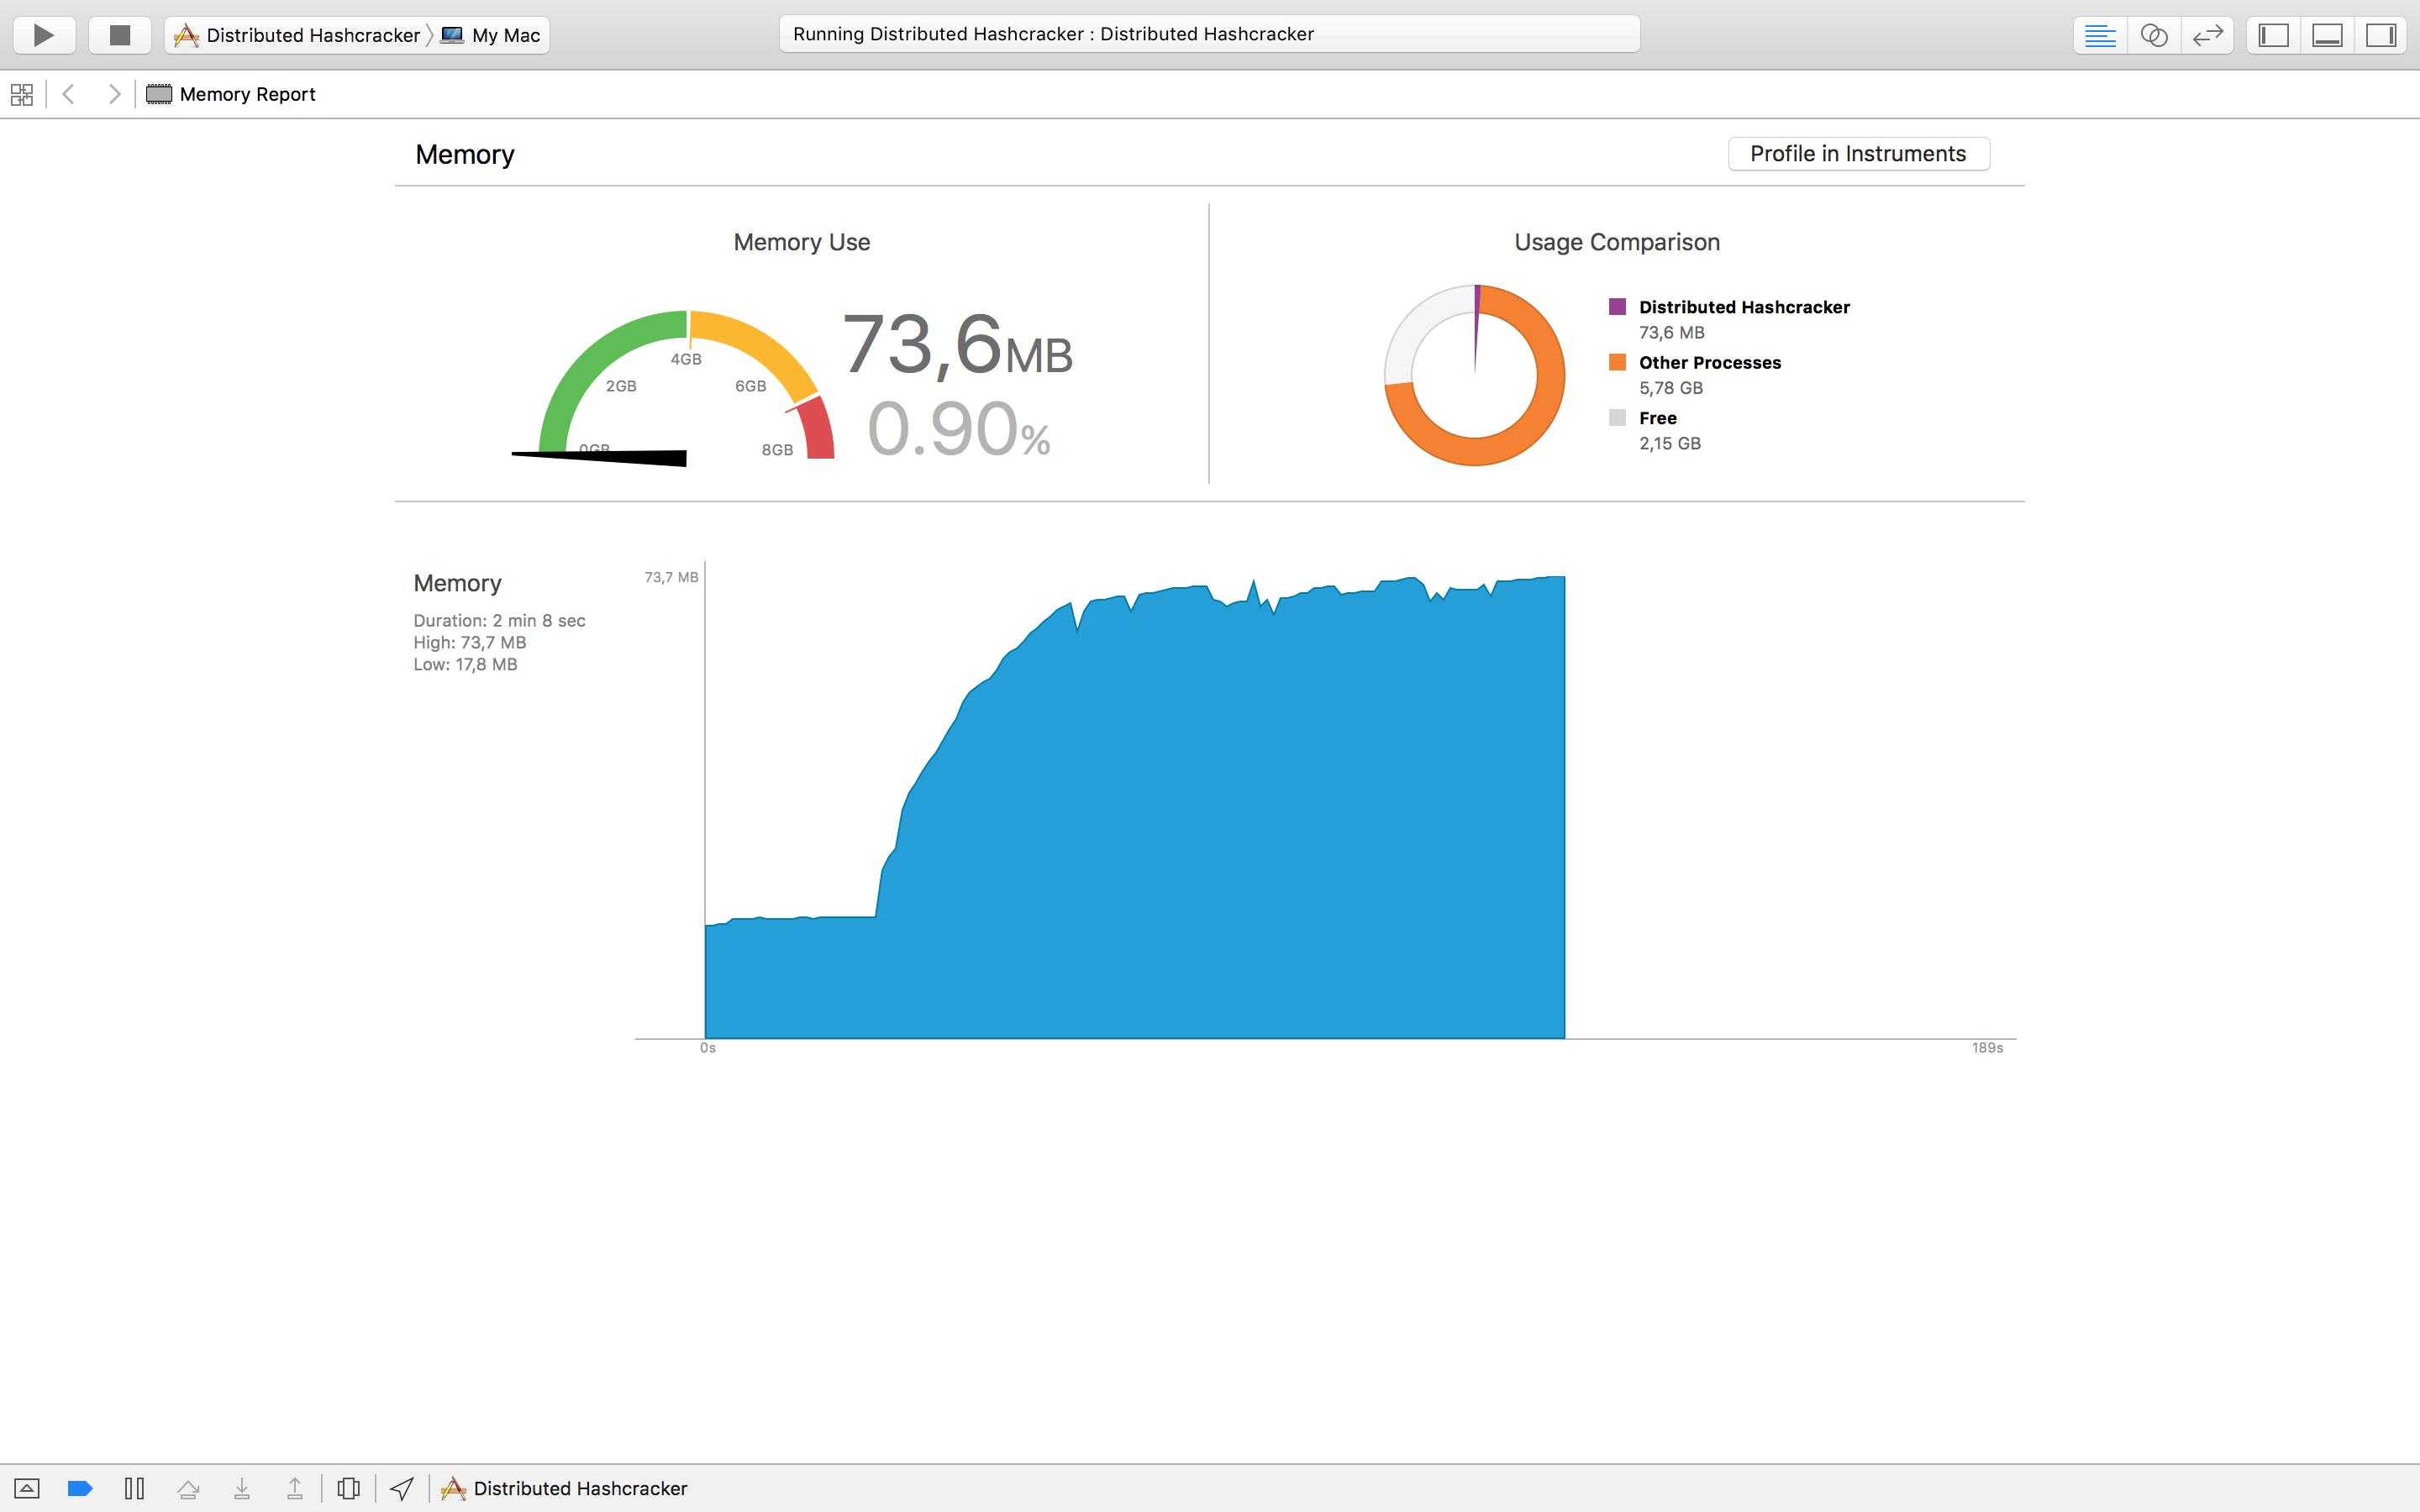
\includegraphics[natwidth=1200pt, natheight=349pt, width=1.0\textwidth]{images/screenshot_ram.png}
	\caption{Verlauf der Arbeitsspeicher-Auslastung während der Laufzeit, gemessen in Xcode.}
	\label{fig:screenshot_ram}
\end{figure}


\section{Benutzeroberfläche}
Nachfolgend wird die Benutzeroberfläche sowie die Interaktion mit dem verteilten System beschrieben. Da primär die Funktionalität der Anwendung im Fokus des Projekts steht, werden nur wenig Interaktionselemente eingesetzt. \\
Die Anwendung wird auf allen Rechnern gestartet, die zum verteilten System zusammengefasst werden. Je nachdem, ob der Rechner als Master oder Worker verwendet werden soll, unterscheidet sich die weitere Interaktion. Die unterschiedlichen Interaktionsmöglichkeiten werden in den folgenden Abschnitten beschrieben. 

\subsection{Master}
Durch Aktivierung des Feldes \enquote{this Mac} im Bereich \emph{Communication Manager} delegiert man den aktuellen Rechner als Master des verteilten Systems. Es gilt zu beachten, dass nur ein Master im verteilten System bestimmt wird. Nachdem diese Option gewählt wurde, wird im Feld \emph{Server Adress} die Adresse des aktuellen Rechners angezeigt. Diese Adresse wird den Workern mitgeteilt (siehe Abschnitt \ref{WorkerGUI}). Auf Abbildung \ref{fig:WindowMaster} lautet die Adresse beispielsweise \emph{127.0.0.1}, da auf dem Rechner kein Domain-Name hinterlegt worden ist. \\
\begin{figure}[!ht]
	\centering
		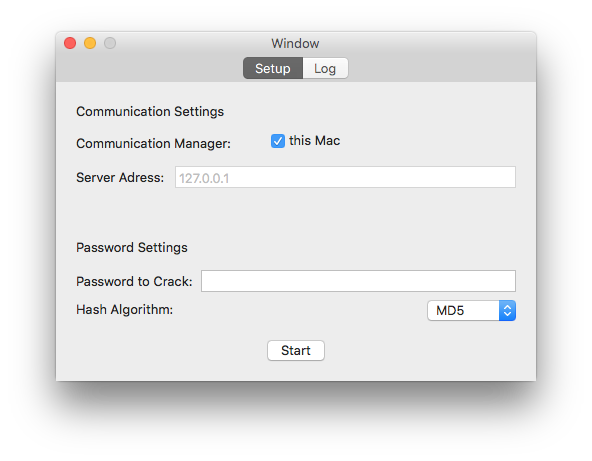
\includegraphics[natwidth=1200pt, natheight=349pt, width=0.6\textwidth]{images/WindowMaster.png}
		\caption{Benutzeroberfläche der implementierten Anwendung als Master der verteilten Anwendung}
	\label{fig:WindowMaster}
\end{figure}
Nach der Konfiguration als Master wird das Passwort festgelegt, welches entschlüsselt werden soll. Dazu wird im Feld \emph{Password to Crack} das gewünschte Passwort eingetragen. Abschließend kann der Hash-Algorithmus ausgewählt werden, mit dem die Hashes erzeugt werden. Die Vorgehensweise zur Entschlüsselung ändert sich dadurch nicht, die Option zur Wahl verschiedener Hash-Algorithmen dient primär zur Messung von Geschwindigkeitsunterschieden. \\

Nach Aktivierung des Start-Buttons steht der Master dem verteilten System zur Verfügung.   


\subsection{Worker}
\label{WorkerGUI}
Nachdem ein Master festgelegt wurde, können beliebig viele Rechner als Worker benutzt werden. Die Rechner müssen sich lediglich im gleichen Netz befinden. \\
Standardmäßig ist die Anwendung nach dem Start als Worker konfiguriert. Dies ist beispielsweise daran zu erkennen, dass die Möglichkeiten zum Eintragen eines Passwortes oder die Auswahl eines Hash-Algorithmus deaktiviert sind (zu erkennen auf Abbildung \ref{fig:WindowWorker}). \\
\begin{figure}[!ht]
	\centering
		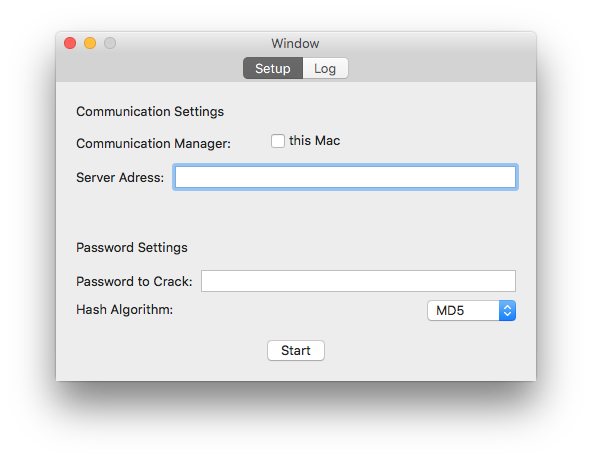
\includegraphics[natwidth=1200pt, natheight=349pt, width=0.6\textwidth]{images/WindowWorker.png}
		\caption{Benutzeroberfläche der implementierten Anwendung als Worker der verteilten Anwendung}
	\label{fig:WindowWorker}
\end{figure}
Damit der Worker mit der Berechnung beginnen kann, muss diesem die Adresse des Masters mitgeteilt werden. Diese kann aus der Anwendung des Masters entnommen werden. Im aktuellen Beispiel würde die Adresse \emph{127.0.0.1}, entnommen aus Abbildung \ref{fig:WindowMaster}, eingetragen werden.\\
Nach der Eintragung der Adresse des Masters kann die Passwortberechnung durch Betätigung des \emph{Start}-Buttons gestartet werden. 



\subsection{Auswertung des Angriffs}
Nach dem Start des Angriffs sind mehrere Beobachtungsmöglichkeiten gegeben. Die erste Möglichkeit ist das Beobachten des Logs. Dieses ist erreichbar, indem das Feld \emph{Log} ausgewählt wird.\\
Das Log stellt Informationen zu verschiedenen Ereignissen bereit. Im aktuellen Beispiel kann aus Abbildung \ref{fig:logView} entnommen werden, dass die Anwendung gestartet und der MD5-Hash-Algorithmus gewählt wurde. Zudem wird der Hash des eingegebenen Passwortes angegeben. Die Information \enquote{showing ChartView} bedeutet, dass die grafische Auswertung des Angriffs aufgerufen wurde.

\begin{figure}[!ht]
	\centering
		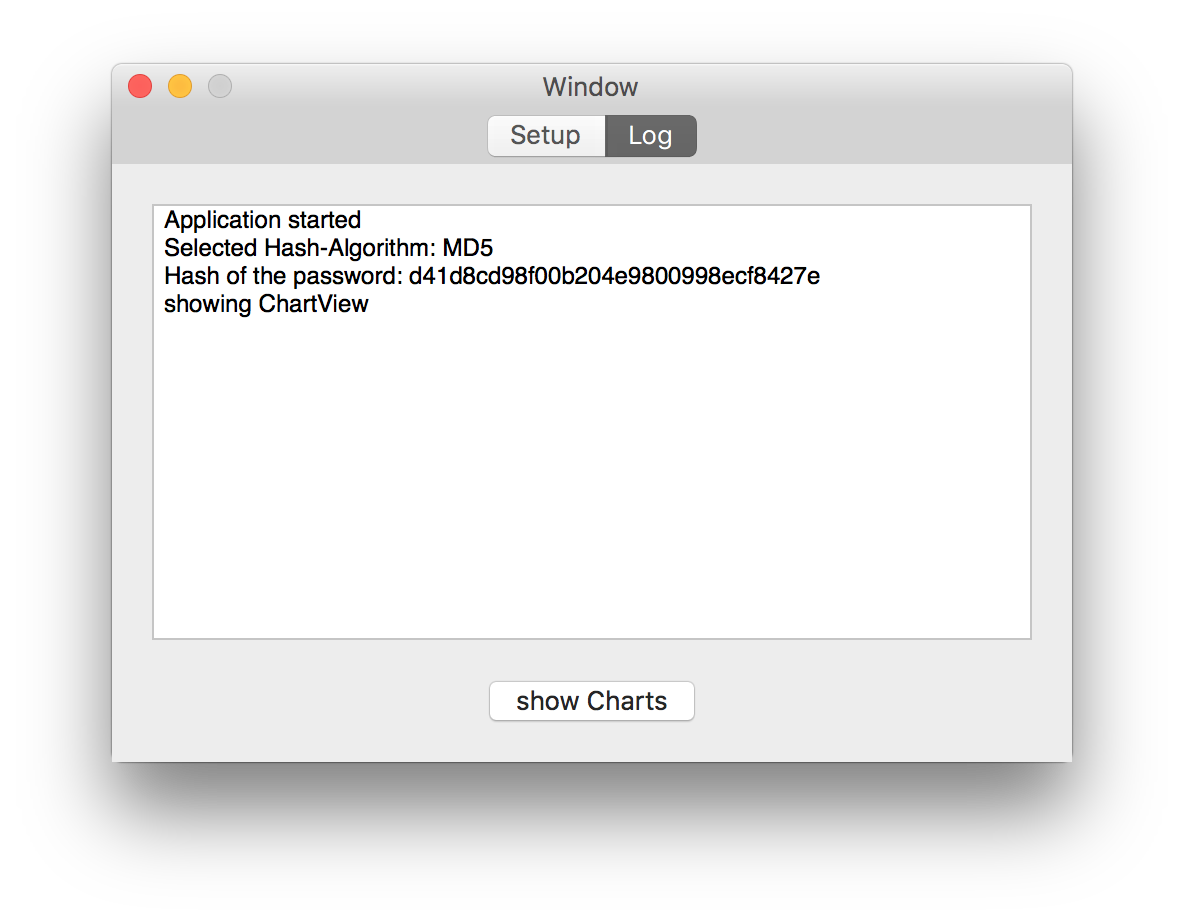
\includegraphics[natwidth=1200pt, natheight=349pt, width=0.6\textwidth]{images/logView.png}
		\caption{Log-Ansicht nach dem Start des BruteForce-Angriffs}
	\label{fig:logView}
\end{figure}

\begin{figure}[!ht]
	\centering
		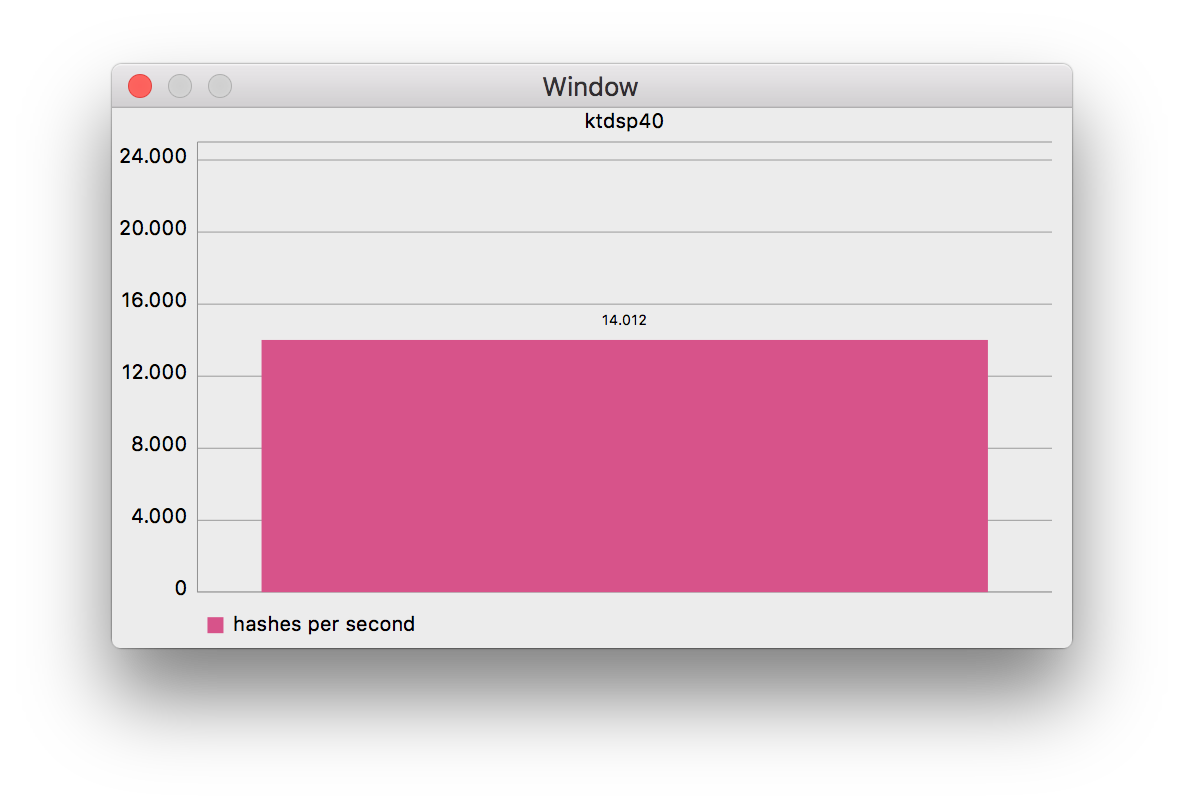
\includegraphics[natwidth=1200pt, natheight=349pt, width=0.6\textwidth]{images/chartView.png}
		\caption{Grafische Darstellung der Quantität an erzeugten Hashes pro Sekunde}
	\label{fig:chartView}
\end{figure}

Die grafische Auswertung des Angriffs ist auf Abbildung \ref{fig:chartView} dargestellt. Die Tabelle stellt in Echtzeit Informationen darüber bereit, wieviele Hashes pro Sekunde durch die jeweiligen Worker erzeugt werden. Auf Grafik \ref{fig:chartView} berechnet aktuell ein Worker 14.012 Hashes pro Sekunde. Die Diagramme zeigen den aktuellen Status der jeweiligen Worker an. Das bedeutet, dass bei Hinzufügen weiterer Worker zum System analog dazu weitere Diagramme angezeigt werden würden. 
